\documentclass[border=10pt]{standalone}
\usepackage{tikz,amsmath}
\usetikzlibrary{positioning,calc,arrows.meta}

% ========== 颜色定义 ==========
\colorlet{myred}{red!80!black}
\colorlet{myblue}{blue!80!black}
\colorlet{mygreen}{green!60!black}

\begin{document}
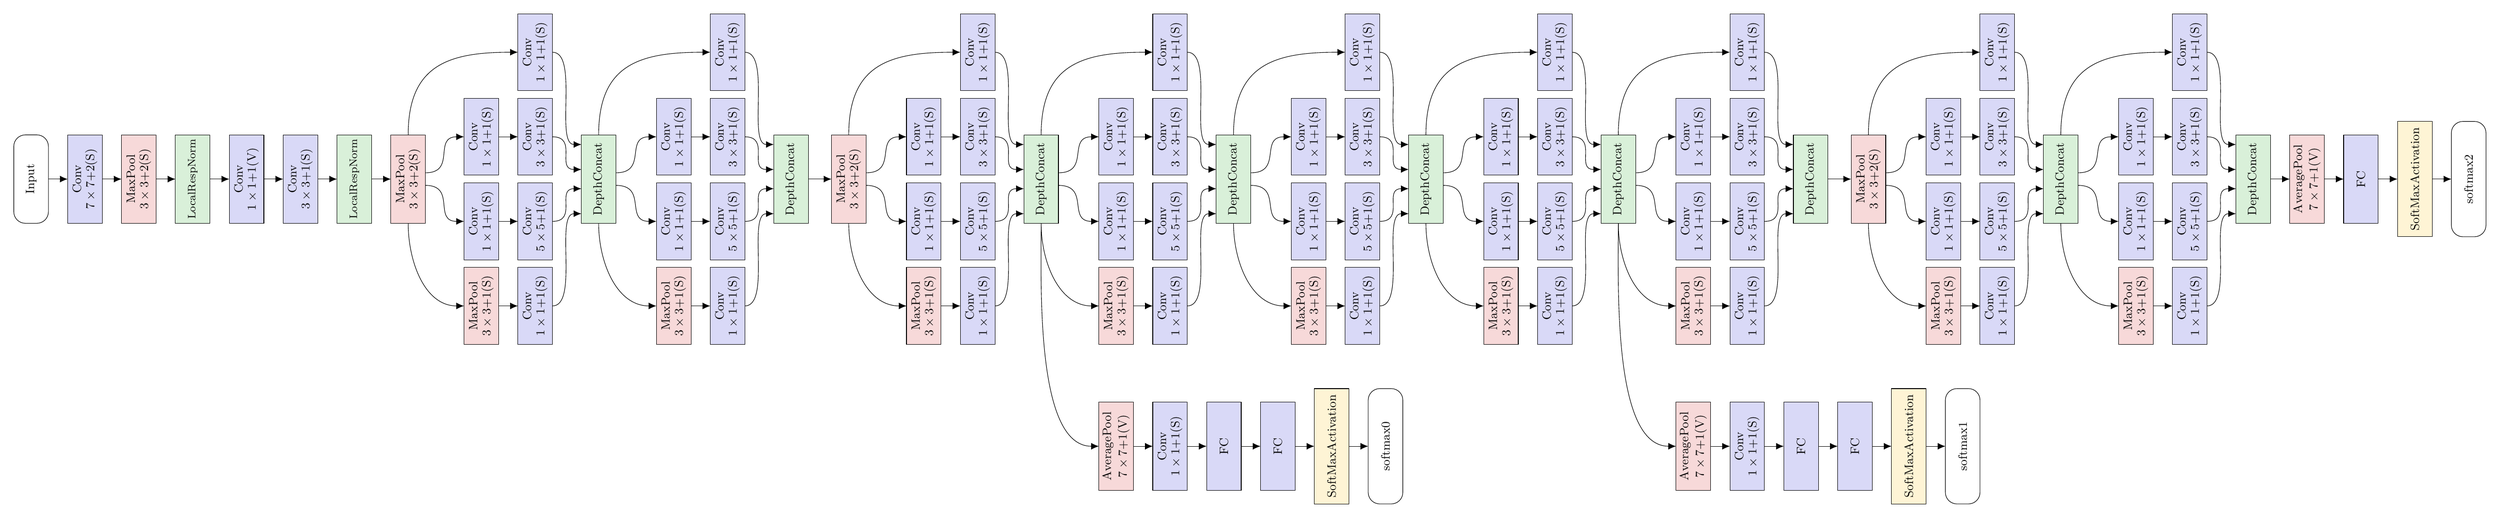
\begin{tikzpicture}[
    font=\small, line join=round,
    every node/.style={outer sep=0pt, inner sep=0pt, align=center},
    w/.style={minimum width=#1},
    h/.style={minimum height=#1},
    >={Latex[length=2mm, width=1.75mm]}
  ]

  % ========== 旋转文字宏（相对原版转 180°）==========
  \newcommand{\rotstack}[1]{\rotatebox{90}{\shortstack{#1}}}

  % ========== Inception 组宏（#1=名前缀，内部结构与原图一致）==========
  \newcommand{\group}[1]{%
    \node[draw, w=.9cm, h=2cm, fill=myblue!15] (#1_a1) {\rotstack{Conv\\$1\times1$+1(S)}};
    \node[draw, w=.9cm, h=2cm, fill=myblue!15, below=.2cm of #1_a1] (#1_a2) {\rotstack{Conv\\$1\times1$+1(S)}};
    \node[draw, w=.9cm, h=2cm, fill=myred!15, below=.2cm of #1_a2] (#1_a3) {\rotstack{MaxPool\\$3\times3$+1(S)}};
    \node[draw, w=.9cm, h=2cm, fill=myblue!15, right=.5cm of #1_a3] (#1_b4) {\rotstack{Conv\\$1\times1$+1(S)}};
    \node[draw, w=.9cm, h=2cm, fill=myblue!15, above=.2cm of #1_b4] (#1_b3) {\rotstack{Conv\\$5\times5$+1(S)}};
    \node[draw, w=.9cm, h=2cm, fill=myblue!15, above=.2cm of #1_b3] (#1_b2) {\rotstack{Conv\\$3\times3$+1(S)}};
    \node[draw, w=.9cm, h=2cm, fill=myblue!15, above=.2cm of #1_b2] (#1_b1) {\rotstack{Conv\\$1\times1$+1(S)}};
    \node[draw, w=.9cm, h=2.3cm, fill=mygreen!15,
          right=.75cm of {$(#1_b2.east)!.5!(#1_b3.east)$}] (#1_c1) {\rotstack{DepthConcat}};
    \draw[->] (#1_a1)--(#1_b2);
    \draw[->] (#1_a2)--(#1_b3);
    \draw[->] (#1_a3)--(#1_b4);
    \draw[->] (#1_b4) to[out=0,in=180,looseness=.7]  ($(#1_c1.west)+(0,-.9)$);
    \draw[->] (#1_b3) to[out=0,in=180,looseness=1.5] ($(#1_c1.west)+(0,-.25)$);
    \draw[->] (#1_b2) to[out=0,in=180,looseness=1.5] ($(#1_c1.west)+(0,.25)$);
    \draw[->] (#1_b1) to[out=0,in=180,looseness=.7]  ($(#1_c1.west)+(0,.9)$);
  }

  % ========== 9 个 Inception 组 ==========
  \begin{scope}[xshift=0cm]    \group{gr1} \end{scope}
  \begin{scope}[xshift=5cm]    \group{gr2} \end{scope}
  \begin{scope}[xshift=11.5cm] \group{gr3} \end{scope}
  \begin{scope}[xshift=16.5cm] \group{gr4} \end{scope}
  \begin{scope}[xshift=21.5cm] \group{gr5} \end{scope}
  \begin{scope}[xshift=26.5cm] \group{gr6} \end{scope}
  \begin{scope}[xshift=31.5cm] \group{gr7} \end{scope}
  \begin{scope}[xshift=38cm]   \group{gr8} \end{scope}
  \begin{scope}[xshift=43cm]   \group{gr9} \end{scope}

  % ========== 组间池化 ==========
  \node[draw, w=.9cm, h=2.3cm, fill=myred!15, right=.6cm of gr2_c1] (m1) {\rotstack{MaxPool\\$3\times3$+2(S)}};
  \node[draw, w=.9cm, h=2.3cm, fill=myred!15, right=.6cm of gr7_c1] (m2) {\rotstack{MaxPool\\$3\times3$+2(S)}};

  % ========== 输出头 ==========
  \node[draw, w=.9cm, h=2.3cm, fill=myred!15, right=.5cm of gr9_c1] (m3) {\rotstack{AveragePool\\$7\times7$+1(V)}};
  \node[draw, w=.9cm, h=2.3cm, fill=myblue!15, right=.5cm of m3] (fc5) {\rotstack{FC}};
  \node[draw, w=.9cm, h=3cm, fill=yellow!50!orange!15, right=.5cm of fc5] (sma3) {\rotstack{SoftMaxActivation}};
  \node[draw, w=.9cm, h=3cm, right=.5cm of sma3, rounded corners=3mm] (sm2) {\rotstack{softmax2}};

  % ========== 辅助分类器 1（gr4 下方）==========
  \node[draw, w=.9cm, h=2.3cm, fill=myred!15, below=1.5cm of gr4_a3] (gr4_a4) {\rotstack{AveragePool\\$7\times7$+1(V)}};
  \node[draw, w=.9cm, h=2.3cm, fill=myblue!15, right=.5cm of gr4_a4] (gr4_b5) {\rotstack{Conv\\$1\times1$+1(S)}};
  \node[draw, w=.9cm, h=2.3cm, fill=myblue!15, right=.5cm of gr4_b5] (fc1) {\rotstack{FC}};
  \node[draw, w=.9cm, h=2.3cm, fill=myblue!15, right=.5cm of fc1] (fc2) {\rotstack{FC}};
  \node[draw, w=.9cm, h=3cm, fill=yellow!50!orange!15, right=.5cm of fc2] (sma1) {\rotstack{SoftMaxActivation}};
  \node[draw, w=.9cm, h=3cm, right=.5cm of sma1, rounded corners=3mm] (sm0) {\rotstack{softmax0}};

  % ========== 辅助分类器 2（gr7 下方）==========
  \node[draw, w=.9cm, h=2.3cm, fill=myred!15, below=1.5cm of gr7_a3] (gr7_a4) {\rotstack{AveragePool\\$7\times7$+1(V)}};
  \node[draw, w=.9cm, h=2.3cm, fill=myblue!15, right=.5cm of gr7_a4] (gr7_b5) {\rotstack{Conv\\$1\times1$+1(S)}};
  \node[draw, w=.9cm, h=2.3cm, fill=myblue!15, right=.5cm of gr7_b5] (fc3) {\rotstack{FC}};
  \node[draw, w=.9cm, h=2.3cm, fill=myblue!15, right=.5cm of fc3] (fc4) {\rotstack{FC}};
  \node[draw, w=.9cm, h=3cm, fill=yellow!50!orange!15, right=.5cm of fc4] (sma2) {\rotstack{SoftMaxActivation}};
  \node[draw, w=.9cm, h=3cm, right=.5cm of sma2, rounded corners=3mm] (sm1) {\rotstack{softmax1}};

  % ========== 前端 stem ==========
  \node[draw, w=.9cm, h=2.3cm, fill=myred!15, left=1cm of {$(gr1_a1.west)!.5!(gr1_a2.west)$}] (m0) {\rotstack{MaxPool\\$3\times3$+2(S)}};
  \node[draw, w=.9cm, h=2.3cm, fill=mygreen!15, left=.5cm of m0] (loc2) {\footnotesize\rotstack{LocalRespNorm}};
  \node[draw, w=.9cm, h=2.3cm, fill=myblue!15, left=.5cm of loc2] (con3) {\rotstack{Conv\\$3\times3$+1(S)}};
  \node[draw, w=.9cm, h=2.3cm, fill=myblue!15, left=.5cm of con3] (con2) {\rotstack{Conv\\$1\times1$+1(V)}};
  \node[draw, w=.9cm, h=2.3cm, fill=mygreen!15, left=.5cm of con2] (loc1) {\footnotesize\rotstack{LocalRespNorm}};
  \node[draw, w=.9cm, h=2.3cm, fill=myred!15, left=.5cm of loc1] (m00) {\rotstack{MaxPool\\$3\times3$+2(S)}};
  \node[draw, w=.9cm, h=2.3cm, fill=myblue!15, left=.5cm of m00] (con1) {\rotstack{Conv\\$7\times7$+2(S)}};
  \node[draw, w=.9cm, h=2.3cm, left=.5cm of con1, rounded corners=3mm] (input) {\rotstack{Input}};

  % ========== 箭头：stem ==========
  \foreach \i/\j in {input/con1, con1/m00, m00/loc1, loc1/con2, con2/con3, con3/loc2, loc2/m0}
    \draw[->] (\i) -- (\j);

  % ========== 箭头：级间四线扇形 ==========
  \foreach \x/\y in {m0/gr1, gr1_c1/gr2, m1/gr3, gr3_c1/gr4, gr4_c1/gr5,
                     gr5_c1/gr6, gr6_c1/gr7, m2/gr8, gr8_c1/gr9} {
    \draw[->] (\x.south) to[out=-90,in=180] (\y_a3.west);
    \draw[->] (\x.north) to[out=90,in=180,looseness=1.3] (\y_b1.west);
    \draw[->] (\x.20) to[out=0,in=180,looseness=1.5] (\y_a1);
    \draw[->] (\x.-20) to[out=0,in=180,looseness=1.5] (\y_a2);
  }

  % ========== 箭头：主链尾段 + 辅助分类器 ==========
  \foreach \x/\y in {gr2_c1/m1, gr7_c1/m2, gr9_c1/m3, m3/fc5, fc5/sma3, sma3/sm2,
                     gr4_a4/gr4_b5, gr4_b5/fc1, fc1/fc2, fc2/sma1, sma1/sm0,
                     gr7_a4/gr7_b5, gr7_b5/fc3, fc3/fc4, fc4/sma2, sma2/sm1}
    \draw[->] (\x) -- (\y);

  % 辅助分类器引出线
  \draw[->] (gr3_c1.south) to[out=-90,in=180,looseness=.7] (gr4_a4.west);
  \draw[->] (gr6_c1.south) to[out=-90,in=180,looseness=.7] (gr7_a4.west);

\end{tikzpicture}
\end{document}